\documentclass[11pt,a4paper]{report}
\usepackage[utf8]{inputenc}
\usepackage[T1]{fontenc}
\usepackage{lmodern}
\IfFileExists{french.ldf}{%
  \usepackage[french]{babel}%
}{%
  \usepackage[english]{babel}%
  \addto\captionsenglish{%
    \renewcommand{\contentsname}{Table des matières}%
    \renewcommand{\listfigurename}{Table des figures}%
    \renewcommand{\listtablename}{Liste des tableaux}%
    \renewcommand{\chaptername}{Chapitre}%
    \renewcommand{\figurename}{Figure}%
    \renewcommand{\tablename}{Tableau}%
    \renewcommand{\bibname}{Bibliographie}%
    \renewcommand{\appendixname}{Annexe}}%
}
\usepackage[a4paper,margin=2.4cm,headheight=14pt]{geometry}
\usepackage{amsmath,amssymb,amsthm,mathtools}
\usepackage{graphicx}
\usepackage{booktabs,tabularx,array,multirow}
\usepackage[table]{xcolor}
\usepackage{tikz}
\usetikzlibrary{arrows.meta,positioning,shapes.geometric,calc,babel}
\usepackage[most]{tcolorbox}
\usepackage{listings}
\usepackage{caption}
\usepackage{float}
\usepackage{enumitem}
\usepackage{fancyhdr}
\usepackage{titlesec}
\usepackage[colorlinks=true,linkcolor=bleu,urlcolor=bleu,citecolor=bleu]{hyperref}

\definecolor{bleu}{RGB}{20,60,130}
\definecolor{gris}{RGB}{245,246,248}
\definecolor{vert}{RGB}{30,120,60}
\definecolor{orange}{RGB}{200,100,20}

\graphicspath{{../figures/}{figures/}}
\setlength{\parindent}{0pt}
\setlength{\parskip}{5pt}
\renewcommand{\arraystretch}{1.25}
\captionsetup{font=small,labelfont=bf}
\newcolumntype{L}{>{\raggedright\arraybackslash}X}

% En-têtes
\pagestyle{fancy}
\fancyhf{}
\fancyhead[L]{\small\nouppercase{\leftmark}}
\fancyfoot[R]{\thepage}
\renewcommand{\headrulewidth}{0.4pt}
\fancypagestyle{plain}{\fancyhf{}\fancyfoot[R]{\thepage}\renewcommand{\headrulewidth}{0pt}}

\ifdefined\chapter
\titleformat{\chapter}[display]{\normalfont\bfseries\color{bleu}}{\large\chaptertitlename\ \thechapter}{6pt}{\LARGE}
\titlespacing*{\chapter}{0pt}{-10pt}{18pt}
\fi
\titleformat{\section}{\normalfont\Large\bfseries\color{bleu}}{\thesection}{0.6em}{}
\titleformat{\subsection}{\normalfont\large\bfseries}{\thesubsection}{0.6em}{}

% Encadrés
\newtcolorbox{demo}[1][]{colback=gris,colframe=bleu!60,boxrule=0.5pt,arc=2pt,left=6pt,right=6pt,top=4pt,bottom=4pt,title={\textbf{Démonstration#1}},fonttitle=\small,coltitle=white,colbacktitle=bleu!70}
\newtcolorbox{retenir}{colback=vert!5,colframe=vert!70,boxrule=0.5pt,arc=2pt,left=6pt,right=6pt,top=4pt,bottom=4pt,title={\textbf{À retenir}},fonttitle=\small,coltitle=white,colbacktitle=vert!70}
\newtcolorbox{question}[1]{colback=orange!5,colframe=orange!80,boxrule=0.5pt,arc=2pt,left=6pt,right=6pt,top=4pt,bottom=4pt,title={\textbf{Question : #1}},fonttitle=\small,coltitle=white,colbacktitle=orange!80}

% Code
\lstset{language=Python,basicstyle=\ttfamily\footnotesize,keywordstyle=\color{bleu}\bfseries,
  commentstyle=\color{vert}\itshape,stringstyle=\color{orange},numbers=left,numberstyle=\tiny\color{gray},
  numbersep=6pt,frame=single,rulecolor=\color{gray!40},backgroundcolor=\color{gris},breaklines=true,
  showstringspaces=false,tabsize=4,columns=fullflexible,keepspaces=true,
  literate={é}{{\'e}}1 {è}{{\`e}}1 {à}{{\`a}}1 {ù}{{\`u}}1 {ê}{{\^e}}1 {ô}{{\^o}}1 {û}{{\^u}}1 {ç}{{\c c}}1
           {î}{{\^i}}1 {â}{{\^a}}1 {É}{{\'E}}1 {À}{{\`A}}1 {σ}{{$\sigma$}}1 {²}{{$^2$}}1 {Δ}{{$\Delta$}}1
           {−}{{-}}1 {√}{{$\surd$}}1 {μ}{{$\mu$}}1 {≈}{{$\approx$}}1 {∈}{{$\in$}}1 {±}{{$\pm$}}1 {→}{{$\to$}}1 {«}{{\guillemotleft}}1 {»}{{\guillemotright}}1}

% Raccourcis
\newcommand{\E}{\mathbb{E}}
\newcommand{\Q}{\mathbb{Q}}
\newcommand{\Var}{\operatorname{Var}}
\newcommand{\Cov}{\operatorname{Cov}}
\newcommand{\Corr}{\operatorname{Corr}}
\newcommand{\Ncal}{\mathcal{N}}
\newcommand{\1}{\mathbf{1}}
\newcommand{\CBS}{C_{BS}}
\newcommand{\vir}{{,}}


\begin{document}

%======================= PAGE DE GARDE =======================
\begin{titlepage}
\thispagestyle{empty}
\begin{minipage}{0.5\textwidth}\small Date : novembre 2026\end{minipage}%
\begin{minipage}{0.5\textwidth}\raggedleft\small Année universitaire : 2026--2027\end{minipage}

\vspace*{1.6cm}
\begin{center}
{\large\bfseries École Supérieure Privée d'Ingénierie et de Technologies (ESPRIT)}\\[0.3cm]
{\normalsize Module : Mathématiques et Assurance}\\[2.2cm]
{\Large Rapport de projet}\\[0.6cm]
\rule{\textwidth}{1pt}\\[0.4cm]
{\huge\bfseries\color{bleu} Modélisation et simulation de Monte-Carlo\\[0.2cm] pour la valorisation d'options financières}\\[0.3cm]
\rule{\textwidth}{1pt}\\[0.6cm]
{\large Le call européen : Black-Scholes, Monte-Carlo et réduction de variance}\\[2.4cm]
\begin{minipage}[t]{0.45\textwidth}\centering
\textbf{Élaboré par :}\\[0.2cm]
Mohamed Derbel\\ Oumaima Mrabet\\ Tasnim Ghodbane\\ Adem Ben Ali\\ Mariem Hamouda
\end{minipage}\hfill
\begin{minipage}[t]{0.45\textwidth}\centering
\textbf{Encadré par :}\\[0.2cm] M. Mohsen Chebbi
\end{minipage}
\end{center}
\end{titlepage}

\pagenumbering{roman}
\tableofcontents
\listoffigures
\listoftables
\cleardoublepage
\pagenumbering{arabic}

\chapter*{Introduction générale}
\addcontentsline{toc}{chapter}{Introduction générale}
\markboth{Introduction générale}{}

La valorisation des produits dérivés est un enjeu central de l'ingénierie financière et de l'assurance : banques et assureurs doivent attribuer un prix à des contrats dont la valeur dépend de l'évolution future d'un actif, le \emph{sous-jacent}. Depuis les travaux de Black, Scholes et Merton (1973), la modélisation stochastique est le cadre de référence.

Ce projet du module \emph{Mathématiques et Assurance} étudie de façon méthodique la \textbf{simulation de Monte-Carlo}. Il procède en deux temps. L'\textbf{option d'achat (call) européenne} sert d'abord de \emph{banc d'essai} idéal : son prix exact $\CBS$ est donné par la formule de Black-Scholes, ce qui permet de mesurer exactement l'erreur de la simulation, sa vitesse de convergence et l'efficacité des techniques de réduction de variance. La méthode, ainsi validée, est ensuite appliquée à une option dépendante du chemin, l'\textbf{option asiatique} à moyenne arithmétique, qui n'a pas de formule fermée : c'est là que Monte-Carlo montre sa vraie valeur pratique.

\paragraph{Démarche.} Le travail suit les quatre étapes de l'énoncé :
\begin{enumerate}[nosep]
  \item modèle de Black-Scholes, résolution log-normale et formule analytique $\CBS$ ;
  \item discrétisation du mouvement brownien géométrique (schéma exact et schéma d'Euler), Monte-Carlo standard (la « méthode de base »), avec des tirages gaussiens générés par la méthode de Box-Muller, et intervalle de confiance à 95\,\% pour $10^3\le N\le 10^6$ ;
  \item optimisation par réduction de variance (variables antithétiques et variable de contrôle), comparaison de l'erreur quadratique moyenne, du gain de variance et du temps de calcul ;
  \item option asiatique : simulation de la grille temporelle complète, prix, sensibilité à la fréquence $M$ et au nombre de trajectoires $N$.
\end{enumerate}

\paragraph{Organisation du rapport.}
Le \textbf{chapitre 1} définit les options et les classe selon deux critères, en commençant par la forme du payoff.
Le \textbf{chapitre 2} présente d'abord les \emph{modèles} du sous-jacent (dont Black-Scholes, démontré en détail), puis les \emph{méthodes} de valorisation, chacune expliquée et illustrée sur le call.
Le \textbf{chapitre 3} réunit la discrétisation, la simulation de Monte-Carlo et la réduction de variance, avec les démonstrations (dont celle du coefficient optimal $c^*$ de la variable de contrôle).
Le \textbf{chapitre 4} applique la méthode à l'option asiatique.
Le \textbf{chapitre 5} explique le code partie par partie.
L'\textbf{annexe A} indique où chaque remarque de l'encadrant a été traitée.

\paragraph{Outils.} Le code est un notebook Jupyter Python (\texttt{numpy}, \texttt{scipy} et \texttt{matplotlib}) entièrement reproductible : chaque partie a son générateur aléatoire à graine fixée, et tous les nombres et figures de ce rapport sont produits par ce notebook. Paramètres de référence :
\[
S_0 = 100,\qquad K = 100,\qquad T = 1 \text{ an},\qquad r = 5\,\%,\qquad \sigma = 20\,\%.
\]

\chapter{Les options : définition et classification}

Ce chapitre répond à deux questions : qu'est-ce qu'une option, et comment la classer ? Il fixe le vocabulaire utilisé dans tout le rapport et justifie le choix de nos deux cas d'étude.

\section{Qu'est-ce qu'une option ?}

Une \textbf{option} est un contrat qui donne à son acheteur le \emph{droit}, sans obligation, d'acheter (\emph{call}) ou de vendre (\emph{put}) un actif sous-jacent à un prix fixé à l'avance, le \emph{strike} $K$, à une date déterminée, l'échéance $T$. L'acheteur paie une \textbf{prime} pour acquérir ce droit : c'est cette prime que l'on cherche à calculer. \textbf{Dans ce projet, nous étudions uniquement le call.}

\begin{figure}[H]
\centering
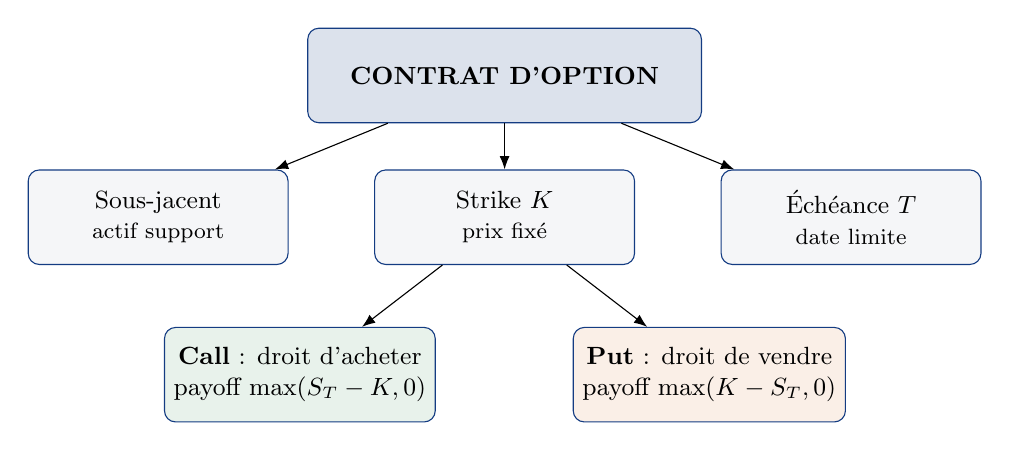
\begin{tikzpicture}[box/.style={draw=bleu,rounded corners,fill=gris,minimum width=3.3cm,minimum height=1.2cm,align=center,font=\small}]
\node[box,fill=bleu!15,minimum width=5cm] (c) at (0,0) {\textbf{CONTRAT D'OPTION}};
\node[box] (s) at (-4.4,-1.8) {Sous-jacent\\ \footnotesize actif support};
\node[box] (k) at (0,-1.8) {Strike $K$\\ \footnotesize prix fixé};
\node[box] (t) at (4.4,-1.8) {Échéance $T$\\ \footnotesize date limite};
\draw[-{Latex}] (c) -- (s); \draw[-{Latex}] (c) -- (k); \draw[-{Latex}] (c) -- (t);
\node[box,fill=vert!10] (call) at (-2.6,-3.8) {\textbf{Call} : droit d'acheter\\ payoff $\max(S_T-K,0)$};
\node[box,fill=orange!10] (put) at (2.6,-3.8) {\textbf{Put} : droit de vendre\\ payoff $\max(K-S_T,0)$};
\draw[-{Latex}] (k) -- (call); \draw[-{Latex}] (k) -- (put);
\end{tikzpicture}
\caption{Structure d'un contrat d'option et payoffs associés.}
\end{figure}

Le \emph{payoff} est ce que reçoit l'acheteur à l'échéance. Pour un call, si $S_T>K$ il achète à $K$ un actif qui vaut $S_T$ et gagne $S_T-K$ ; sinon il n'exerce pas et reçoit $0$.

\section{Deux critères de classification}

Au-delà du sens du droit (call ou put), une option se classe selon \textbf{deux critères indépendants}. Nous plaçons en premier le critère de la \emph{forme du payoff}, car c'est lui qui décide de la méthode de valorisation utilisable : formule exacte pour une option vanille, simulation pour une option dépendante du chemin.

\begin{table}[H]
\centering\small
\begin{tabularx}{\textwidth}{>{\bfseries}p{3.4cm}p{3.6cm}L}
\toprule
Critère & Types & Idée \\
\midrule
Critère 1 : forme du payoff & Vanille / Exotique & Vanille : le payoff ne dépend que de $S_T$. Exotique : règle plus complexe ; en particulier \emph{path-dependent} quand le payoff dépend de la trajectoire (moyenne, barrière, extremum). \\
Critère 2 : instant d'exercice & Européenne / Bermudéenne / Américaine & Européenne : seulement à $T$. Bermudéenne : à des dates fixées à l'avance. Américaine : à tout instant jusqu'à $T$. \\
\bottomrule
\end{tabularx}
\caption{Les deux critères de classification des options.}
\label{tab:criteres}
\end{table}

\subsection{Critère 1 : la forme du payoff}

Une option \textbf{vanille} a un payoff qui dépend du seul prix final $S_T$ : $(S_T-K)^+$ pour le call (on note $x^+ = \max(x,0)$). Une option \textbf{exotique} a un payoff plus riche. Le point décisif pour ce projet est la notion de \textbf{dépendance au chemin} :
\begin{itemize}[nosep]
\item si le payoff ne dépend que de $S_T$, il suffit de connaître la \emph{loi de $S_T$} pour calculer le prix (une seule variable aléatoire) ;
\item si le payoff dépend de $S_{t_1},\dots,S_{t_M}$, il faut connaître la \emph{loi jointe} de toute la trajectoire : c'est un problème en dimension $M$, où les formules fermées disparaissent en général.
\end{itemize}

\begin{table}[H]
\centering\small
\begin{tabularx}{\textwidth}{>{\bfseries}p{2.4cm}p{4.6cm}L}
\toprule
Famille & Payoff (call) & Particularité \\
\midrule
Vanille & $(S_T-K)^+$ & Dépend de $S_T$ seulement. Formule de Black-Scholes. \textbf{Notre cas d'étude.} \\
Asiatique & $(A-K)^+$, $A = \frac1M\sum_{j=1}^M S_{t_j}$ & \emph{Path-dependent} : moyenne sur la trajectoire. Étudiée au chapitre~\ref{ch:asiatique}. \\
À barrière & $(S_T-K)^+\1_{\{\max_t S_t < B\}}$ & \emph{Path-dependent} : s'annule si la barrière $B$ est franchie. \\
Lookback & $S_T - \min_{t\le T}S_t$ & \emph{Path-dependent} : dépend de l'extremum atteint. \\
Digitale & $\1_{\{S_T>K\}}$ & Payoff discontinu (tout ou rien). \\
Panier & $\big(\sum_i w_iS_T^{(i)} - K\big)^+$ & Plusieurs sous-jacents. \\
\bottomrule
\end{tabularx}
\caption{Options vanilles et principales familles d'options exotiques.}
\end{table}

\subsection{Critère 2 : l'instant d'exercice}

\begin{figure}[H]
\centering
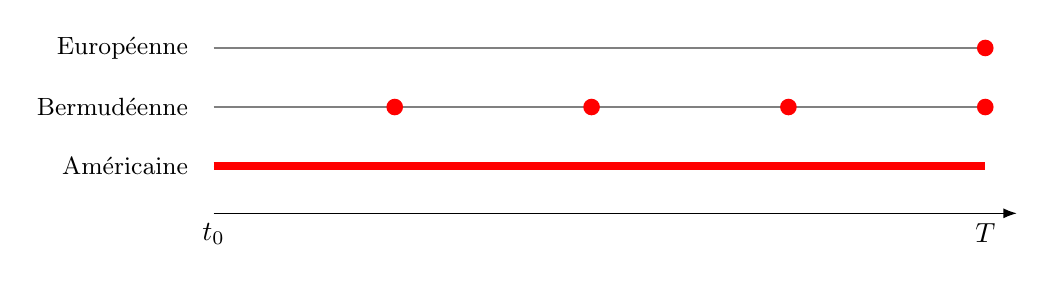
\begin{tikzpicture}[x=1cm,y=0.75cm]
\foreach \y/\n in {2/Européenne,1/Bermudéenne,0/Américaine}{\node[left,font=\small] at (0,\y) {\n}; \draw[gray] (0.2,\y) -- (10,\y);}
\fill[red] (10,2) circle (3pt);
\foreach \x in {2.5,5,7.5,10} \fill[red] (\x,1) circle (3pt);
\draw[red,line width=3pt] (0.2,0) -- (10,0);
\draw[-{Latex}] (0.2,-0.8) -- (10.4,-0.8); \node[below] at (0.2,-0.8) {$t_0$}; \node[below] at (10,-0.8) {$T$};
\end{tikzpicture}
\caption{Instants d'exercice possibles (en rouge) : à $T$ seulement, à des dates discrètes, à tout instant.}
\end{figure}

Plus de liberté d'exercice vaut plus cher ; à payoff identique :
\[
V_{\text{européenne}} \le V_{\text{bermudéenne}} \le V_{\text{américaine}}.
\]
Pour un call sur un actif sans dividende, l'exercice anticipé n'est jamais optimal : le call américain vaut alors le call européen.

\subsection{Croisement des deux critères}

\begin{table}[H]
\centering\small
\begin{tabularx}{\textwidth}{>{\bfseries}p{2.6cm}LL}
\toprule
 & Vanille & Exotique \\
\midrule
Européenne & \textbf{Call européen} (Black-Scholes) $\leftarrow$ \textbf{notre cas d'étude} & Asiatique (chapitre~\ref{ch:asiatique}), barrière, digitale \\
Bermudéenne & Call ou put bermudéen, swaption bermudéenne & Variantes exotiques à dates d'exercice discrètes \\
Américaine & Put américain sur action & Asiatique ou barrière américaine (rares) \\
\bottomrule
\end{tabularx}
\caption{Croisement des deux critères : exemples.}
\end{table}

\textbf{Précision importante.} « Européenne » et « asiatique » ne s'opposent pas sur le même critère : « européenne » décrit l'\emph{instant d'exercice} (critère 2), « asiatique » décrit la \emph{forme du payoff} (critère 1). Une option asiatique peut donc être \emph{à exercice européen} tout en ayant un payoff qui porte sur une moyenne.

\section{Notre cas d'étude : le call européen}

Selon les deux critères, le call européen est une option \textbf{vanille} (critère 1) à \textbf{exercice européen} (critère 2). C'est le cas le plus simple, et c'est précisément ce qui en fait un bon banc d'essai :
\begin{itemize}[nosep]
\item son payoff $(S_T-K)^+$ ne dépend que de $S_T$, dont la loi est connue exactement dans le modèle de Black-Scholes ;
\item il a donc un \textbf{prix exact}, $\CBS = 10{,}4506$ avec nos paramètres (chapitre 2) ;
\item on peut ainsi mesurer exactement l'erreur de Monte-Carlo, vérifier l'intervalle de confiance et comparer objectivement les techniques de réduction de variance (chapitre 3).
\end{itemize}
Une fois la méthode validée sur ce cas, elle pourra être appliquée en toute confiance aux options sans formule fermée, comme l'option asiatique (chapitre~\ref{ch:asiatique}).

\begin{table}[H]
\centering\small
\begin{tabularx}{\textwidth}{>{\bfseries}p{3.2cm}L}
\toprule
Payoff & $(S_T-K)^+$ : on reçoit $S_T-K$ si $S_T>K$, sinon $0$ \\
Exercice & Uniquement à l'échéance $T$ \\
Dépend de & Prix final $S_T$ seulement \\
Prix exact & Formule de Black-Scholes : $\CBS = 10{,}4506$ \\
Rôle dans le projet & Référence pour valider et optimiser Monte-Carlo \\
Usage typique & Spéculation à la hausse, couverture (actions, indices, devises) \\
\bottomrule
\end{tabularx}
\caption{Fiche du call européen ($S_0=K=100$, $T=1$, $r=5\,\%$, $\sigma=20\,\%$).}
\end{table}

\chapter{Valoriser une option : d'abord le modèle, ensuite la méthode}

\section{Principe commun : l'espérance risque-neutre}

Évaluer une option, c'est calculer l'\textbf{espérance actualisée de son payoff sous la probabilité risque-neutre} $\Q$ :
\[
V_0 = e^{-rT}\,\E_\Q[\text{Payoff}].
\]
Deux ingrédients, à ne pas confondre, interviennent \emph{dans cet ordre} :
\begin{enumerate}[nosep]
\item \textbf{le modèle} dit \emph{comment évolue le prix du sous-jacent} (volatilité constante ou aléatoire, sauts\dots) ; il fixe la loi de $S_T$ ou de la trajectoire, donc ce que vaut l'espérance ;
\item \textbf{la méthode} dit \emph{comment on calcule numériquement cette espérance} une fois le modèle choisi (formule, EDP, arbre, simulation\dots).
\end{enumerate}
On choisit donc toujours le modèle d'abord : sans modèle, il n'y a pas d'espérance à calculer. Une même méthode (Monte-Carlo) peut servir pour tous les modèles, et un même modèle (Black-Scholes) peut être traité par toutes les méthodes.

\section{Les modèles du sous-jacent}

\begin{table}[H]
\centering\small
\begin{tabularx}{\textwidth}{>{\bfseries}p{2.7cm}p{6.2cm}L}
\toprule
Modèle & Dynamique sous $\Q$ & Prix du call européen \\
\midrule
Black-Scholes (GBM) & $dS_t = rS_tdt + \sigma S_tdW_t$ & Formule fermée \\
Volatilité locale (Dupire) & $dS_t = rS_tdt + \sigma(t,S_t)S_tdW_t$ & EDP ou Monte-Carlo \\
Heston & $dS_t = rS_tdt + \sqrt{v_t}S_tdW^1_t$,\ \ $dv_t = \kappa(\theta-v_t)dt + \xi\sqrt{v_t}dW^2_t$ & Semi-fermée (Fourier) \\
Merton (sauts) & $\frac{dS_t}{S_{t^-}} = (r-\lambda\kappa)dt + \sigma dW_t + (J-1)dN_t$ & Série de prix BS \\
Vasicek / CIR & taux court $dr_t = a(b-r_t)dt + \sigma_r r_t^{\gamma}dW_t$ & Hors cadre (options sur taux) \\
\bottomrule
\end{tabularx}
\caption{Modèles de dynamique du sous-jacent et méthodes disponibles.}
\label{tab:modeles}
\end{table}

\begin{itemize}[nosep]
\item \textbf{Black-Scholes} : volatilité constante, trajectoires continues. C'est le modèle le plus simple et le seul qui donne une formule fermée pour l'européenne. \emph{C'est notre cadre.}
\item \textbf{Dupire} : la volatilité dépend du temps et du prix, ce qui permet de reproduire exactement les prix d'options observés sur le marché.
\item \textbf{Heston} : la variance $v_t$ est elle-même aléatoire (retour à la moyenne $\theta$ à la vitesse $\kappa$, volatilité de la volatilité $\xi$) ; elle explique le « smile » de volatilité.
\item \textbf{Merton} : ajoute des sauts (processus de Poisson $N_t$ d'intensité $\lambda$, amplitude $J$) pour représenter les krachs.
\item \textbf{Vasicek / CIR} : modèles de \emph{taux} d'intérêt, hors de notre cadre (taux $r$ constant).
\end{itemize}
Quel que soit le modèle, Monte-Carlo s'applique de la même façon : seule la simulation de $S_T$ change. Nous n'implémentons que Black-Scholes, que nous détaillons maintenant.

\section{Le modèle de Black-Scholes : le prix exact de référence}

\subsection{L'équation différentielle stochastique}
Sous la mesure risque-neutre, le prix du sous-jacent suit le mouvement brownien géométrique
\[
dS_t = r\,S_t\,dt + \sigma\,S_t\,dW_t ,\qquad S_0 \text{ donné},
\]
où $W$ est un mouvement brownien : $W_0=0$, trajectoires continues, accroissements indépendants et $W_t-W_s\sim\Ncal(0,t-s)$. Le terme $rS_tdt$ est la tendance (taux sans risque) et $\sigma S_tdW_t$ le bruit (volatilité $\sigma$).

\subsection{Existence et unicité}
Les coefficients $a(x) = rx$ et $b(x) = \sigma x$ sont lipschitziens et à croissance linéaire :
$|a(x)-a(y)| \le r|x-y|$, $|b(x)-b(y)|\le\sigma|x-y|$, $|a(x)|+|b(x)|\le (r+\sigma)(1+|x|)$.
Le théorème d'existence et d'unicité des EDS garantit donc une solution forte unique, continue, pour tout $S_0$.
\emph{Probabilité réelle ou risque-neutre ?} Sous la probabilité réelle la tendance est $\mu$ ; pour valoriser, le théorème de Girsanov permet de passer à $\Q$ sous laquelle la tendance devient $r$.

\subsection{Résolution : la loi log-normale}
\begin{demo}[ — solution de l'EDS par le lemme d'Itô]
On pose $X_t = \ln S_t$, soit $f(s)=\ln s$, $f'(s) = 1/s$, $f''(s) = -1/s^2$. Le lemme d'Itô donne
\[
dX_t = f'(S_t)dS_t + \tfrac12f''(S_t)(dS_t)^2 = \frac{dS_t}{S_t} - \frac{(dS_t)^2}{2S_t^2}.
\]
Comme $(dW_t)^2 = dt$ et $dt\,dW_t = (dt)^2 = 0$, on a $(dS_t)^2 = \sigma^2S_t^2dt$, d'où
\[
dX_t = \Big(r-\frac{\sigma^2}{2}\Big)dt + \sigma dW_t.
\]
Les coefficients étant constants, on intègre entre $0$ et $T$, puis on écrit $W_T = \sqrt T Z$ avec $Z\sim\Ncal(0,1)$ :
\[
\boxed{S_T = S_0\exp\Big[\Big(r-\frac{\sigma^2}2\Big)T + \sigma\sqrt T\,Z\Big]}
\qquad\Longrightarrow\qquad \ln S_T\sim\Ncal\Big(\ln S_0+\Big(r-\frac{\sigma^2}2\Big)T,\ \sigma^2T\Big).
\]
\end{demo}

$S_T$ est donc \textbf{log-normale}. Le terme $-\sigma^2/2$ est la \emph{correction d'Itô} : comme $\E[e^{aZ}] = e^{a^2/2}$, on obtient
$\E[S_T] = S_0e^{(r-\sigma^2/2)T}e^{\sigma^2T/2} = S_0e^{rT}$. L'actif actualisé $e^{-rt}S_t$ est d'espérance constante (c'est une martingale) : c'est la propriété qui définit la mesure risque-neutre.

\subsection{La formule de Black-Scholes}
\begin{demo}[ — formule du call européen]
On veut $C = e^{-rT}\E[(S_T-K)^+]$.

\emph{a) Événement d'exercice.} $S_T>K \iff Z>-d_2$, avec $d_2 = \dfrac{\ln(S_0/K)+(r-\sigma^2/2)T}{\sigma\sqrt T}$. Donc $\Q(S_T>K) = N(d_2)$.

\emph{b) Découpage.} $\E[(S_T-K)^+] = \E[S_T\1_{\{Z>-d_2\}}] - K\,N(d_2)$.

\emph{c) Premier terme : on complète le carré.} En utilisant $\sigma\sqrt Tz - \frac{z^2}{2} = -\frac12(z-\sigma\sqrt T)^2 + \frac{\sigma^2T}{2}$ :
\[
\E[S_T\1_{\{Z>-d_2\}}] = S_0e^{(r-\frac{\sigma^2}{2})T}\!\int_{-d_2}^{\infty}\! e^{\sigma\sqrt Tz}\frac{e^{-z^2/2}}{\sqrt{2\pi}}dz
= S_0e^{rT}\!\int_{-d_2}^{\infty}\!\frac{e^{-(z-\sigma\sqrt T)^2/2}}{\sqrt{2\pi}}dz = S_0e^{rT}N(d_2+\sigma\sqrt T).
\]
\emph{d) Conclusion.} Avec $d_1 = d_2+\sigma\sqrt T$ :
\[
\boxed{\CBS = S_0N(d_1) - Ke^{-rT}N(d_2)},\qquad d_1 = \frac{\ln(S_0/K)+(r+\sigma^2/2)T}{\sigma\sqrt T},\quad d_2 = d_1-\sigma\sqrt T.
\]
\end{demo}

$N(\cdot)$ est la fonction de répartition de $\Ncal(0,1)$ et $N(d_2)$ la probabilité risque-neutre de finir dans la monnaie.

\textbf{Exemple chiffré (référence de tout le projet).} $d_1 = (0 + 0{,}07)/0{,}2 = 0{,}35$, $d_2 = 0{,}15$, $N(d_1)\approx 0{,}6368$, $N(d_2)\approx0{,}5596$ :
\[
\CBS = 100\times0{,}6368 - 100\,e^{-0{,}05}\times0{,}5596 = \mathbf{10{,}4506}.
\]


\subsection{L'EDP de Black-Scholes et la formule de Feynman-Kac}
Le prix $V(t,S)$ vérifie aussi une équation aux dérivées partielles. En appliquant Itô à $e^{-rt}V(t,S_t)$, qui doit être une martingale sous $\Q$, le terme en $dt$ doit s'annuler :
\[
\frac{\partial V}{\partial t} + \frac12\sigma^2S^2\frac{\partial^2V}{\partial S^2} + rS\frac{\partial V}{\partial S} - rV = 0,\qquad V(T,S) = (S-K)^+.
\]
Réciproquement, la \textbf{formule de Feynman-Kac} dit que la solution de cette EDP s'écrit comme une espérance :
$V(t,S) = e^{-r(T-t)}\E_\Q[(S_T-K)^+\mid S_t = S]$.
\emph{Résoudre l'EDP (analyse) et calculer l'espérance (probabilités) sont donc deux façons de résoudre le même problème} : c'est ce qui justifie les différentes méthodes ci-dessous.

\section{Les méthodes de valorisation}

Le modèle étant fixé, il reste à calculer l'espérance. Nous détaillons chaque méthode : principe, mise en œuvre, application au call européen, limites.

\subsection{Formule fermée}
\textbf{Principe.} Calculer l'intégrale exactement, comme dans la démonstration ci-dessus.
\textbf{Call européen :} oui, c'est $\CBS$, instantanée et exacte.
\textbf{Limite :} n'existe que dans des cas très particuliers (modèle simple, payoff qui ne dépend que de $S_T$). Dès que le payoff dépend de toute la trajectoire, il n'y a en général plus de formule.

\subsection{EDP et différences finies}
\textbf{Principe.} On résout numériquement l'EDP de Black-Scholes sur une grille $S_i = i\Delta S$ ($0\le i\le n_S$, $S_{\max} = 2K$), $t_n = n\Delta t$ ($0\le n\le n_t$), en partant de la condition finale $V(T,S) = (S-K)^+$ et en remontant le temps. Les dérivées sont remplacées par des différences :
\[
\frac{\partial V}{\partial S}\approx\frac{V_{i+1}-V_{i-1}}{2\Delta S},\qquad \frac{\partial^2V}{\partial S^2}\approx\frac{V_{i+1}-2V_i+V_{i-1}}{\Delta S^2}.
\]
\textbf{Schéma implicite.} Ces dérivées sont prises au temps inconnu $t_n$, ce qui donne à chaque pas un système tridiagonal
\[
a_iV^n_{i-1} + b_iV^n_i + c_iV^n_{i+1} = V^{n+1}_i,\quad a_i = \tfrac{\Delta t}{2}(ri - \sigma^2i^2),\ b_i = 1+\Delta t(\sigma^2i^2+r),\ c_i = -\tfrac{\Delta t}{2}(\sigma^2i^2+ri),
\]
avec les conditions aux bords $V(t,0)=0$ et $V(t,S_{\max}) = S_{\max}-Ke^{-r(T-t)}$. On le résout en $O(n_S)$ opérations par l'algorithme de Thomas. Le schéma implicite est inconditionnellement stable (contrairement au schéma explicite, qui impose $\Delta t \lesssim \Delta S^2/(\sigma^2S_{\max}^2)$).


\textbf{Atout :} l'erreur diminue quand on affine la grille, et en dimension 1 l'EDP est \emph{plus efficace} que Monte-Carlo.
\textbf{Limite :} \emph{malédiction de la dimension} : avec $d$ variables d'état (plusieurs sous-jacents, volatilité aléatoire, payoff dépendant du chemin\dots) et $n$ points par axe, la grille a $n^d$ nœuds.

\subsection{Arbre binomial de Cox-Ross-Rubinstein}
\textbf{Principe.} On découpe $[0,T]$ en $n$ pas. À chaque pas, le prix est multiplié par $u = e^{\sigma\sqrt{\Delta t}}$ ou par $d = 1/u$. La probabilité de hausse
\[
p = \frac{e^{r\Delta t}-d}{u-d}
\]
est choisie pour que $\E[S_{t+\Delta t}\mid S_t] = S_te^{r\Delta t}$ (neutralité au risque). On calcule les payoffs aux $n+1$ feuilles, puis on remonte : $V = e^{-r\Delta t}\big(pV_{\text{haut}}+(1-p)V_{\text{bas}}\big)$. Quand $n\to\infty$, la loi de $S_T$ dans l'arbre tend vers la log-normale (théorème central limite) et le prix tend vers $\CBS$.


\textbf{Atouts :} très intuitif, et c'est la méthode naturelle pour les options \emph{américaines} (à chaque nœud on compare la valeur de continuation à la valeur d'exercice).
\textbf{Limite :} convergence lente et oscillante en $O(1/n)$ ; et si le payoff dépend du chemin, l'arbre ne se « recombine » plus et il faut suivre les $2^n$ chemins.

\subsection{Monte-Carlo}
\textbf{Principe.} Remplacer l'espérance par une moyenne de payoffs simulés (loi des grands nombres), et mesurer l'erreur par un intervalle de confiance (théorème central limite). La méthode est détaillée au chapitre 3.
\textbf{Call européen :} oui ; ici la formule exacte permet de mesurer précisément son erreur.
\textbf{Atout :} l'erreur reste en $\sigma_X/\sqrt N$ \emph{quelle que soit la dimension} du problème, et la méthode s'adapte à n'importe quel modèle ou payoff.
\textbf{Limite :} convergence lente en $1/\sqrt N$, d'où la réduction de variance.

\subsection{Transformée de Fourier (Carr-Madan)}
\textbf{Principe.} Si l'on connaît la fonction caractéristique $\varphi(u) = \E[e^{iu\ln S_T}]$ (c'est le cas pour Black-Scholes, Heston, Merton), le prix d'un call amorti $e^{\alpha k}C(k)$, $k = \ln K$, a une transformée de Fourier explicite :
\[
\psi(v) = \frac{e^{-rT}\varphi\big(v-(\alpha+1)i\big)}{\alpha^2+\alpha-v^2+i(2\alpha+1)v},\qquad C(k) = \frac{e^{-\alpha k}}{\pi}\int_0^\infty \Re\big(e^{-ivk}\psi(v)\big)\,dv,
\]
calculée pour tous les strikes en une seule FFT.
\textbf{Call européen :} oui, si $\varphi$ est connue ; très rapide pour calibrer un modèle sur de nombreux strikes.
\textbf{Limite :} exige une fonction caractéristique connue, et ne s'applique qu'aux payoffs qui dépendent de $S_T$ seulement.

\subsection{Synthèse comparative}

\begin{table}[H]
\centering\small
\begin{tabularx}{\textwidth}{>{\bfseries}p{2.6cm}LLL}
\toprule
Méthode & Call européen & Atout & Limite principale \\
\midrule
Formule fermée & Oui : Black-Scholes, exacte & Instantanée & Cas très particuliers \\
EDP (différences finies) & Oui, converge vers $\CBS$ & Très efficace en dimension 1 & Malédiction de la dimension \\
Arbre CRR & Oui, converge en $O(1/n)$ & Intuitif, options américaines & Lent, oscillant en $O(1/n)$ \\
Monte-Carlo & Oui, IC $\pm0{,}029$ ($N=10^6$) & Indépendant de la dimension & Erreur en $1/\sqrt N$ \\
Fourier (Carr-Madan) & Oui si $\varphi$ connue & Tous les strikes en une FFT & Exige $\varphi$ \\
\bottomrule
\end{tabularx}
\caption{Synthèse des méthodes de valorisation appliquées au call européen.}
\end{table}

\begin{retenir}
Pour le call européen, toutes les méthodes fonctionnent et la formule fermée est imbattable : elle sert de \emph{référence}. Monte-Carlo est la plus lente ici, mais c'est la seule dont l'erreur ne dépend pas de la dimension du problème. D'où notre démarche : \textbf{valider et optimiser Monte-Carlo sur le call européen}, là où l'on connaît la bonne réponse.
\end{retenir}

\chapter{Monte-Carlo et réduction de variance (call européen)}

Ce chapitre réunit la méthode de Monte-Carlo \emph{de base} et son \emph{optimisation} par réduction de variance. Le call européen sert de banc d'essai : comme on connaît $\CBS = 10{,}4506$, on peut mesurer exactement l'erreur de la simulation.

\section{Principe et algorithme}

Le prix est une espérance : $C = \E[Y]$ avec $Y = e^{-rT}(S_T-K)^+$ (on garde les notations du code). Monte-Carlo la remplace par la moyenne de $N$ simulations indépendantes :
\[
\hat C = \frac1N\sum_{i=1}^N Y_i,\qquad Y_i = e^{-rT}\big(S_T^{(i)}-K\big)^+,\qquad S_T^{(i)} = S_0\exp\Big[\Big(r-\frac{\sigma^2}2\Big)T+\sigma\sqrt T\,Z_i\Big].
\]

\begin{figure}[H]
\centering
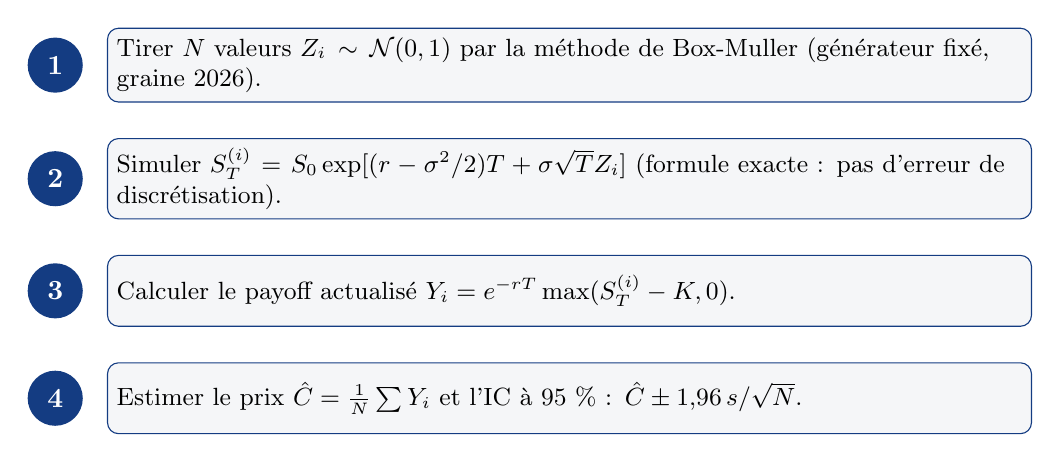
\begin{tikzpicture}[node distance=0.45cm,box/.style={draw=bleu,rounded corners,fill=gris,text width=11.5cm,minimum height=0.9cm,align=left,font=\small},num/.style={circle,fill=bleu,text=white,font=\bfseries,minimum size=0.7cm}]
\node[box] (a) {Tirer $N$ valeurs $Z_i\sim\Ncal(0,1)$ par la méthode de Box-Muller (générateur fixé, graine 2026).};
\node[box,below=of a] (b) {Simuler $S_T^{(i)} = S_0\exp[(r-\sigma^2/2)T+\sigma\sqrt TZ_i]$ (formule exacte : pas d'erreur de discrétisation).};
\node[box,below=of b] (c) {Calculer le payoff actualisé $Y_i = e^{-rT}\max(S_T^{(i)}-K,0)$.};
\node[box,below=of c] (d) {Estimer le prix $\hat C = \frac1N\sum Y_i$ et l'IC à 95 \% : $\hat C\pm1{,}96\,s/\sqrt N$.};
\foreach \n/\k in {a/1,b/2,c/3,d/4} \node[num,left=0.3cm of \n] {\k};
\end{tikzpicture}
\caption{Algorithme de Monte-Carlo en quatre étapes (méthode de base).}
\end{figure}

\section{Étape 1 : générateur fixé et méthode de Box-Muller}\label{sec:bm}

\paragraph{Le générateur est fixé.} Le générateur de NumPy produit des nombres \emph{uniformes} sur $[0,1[$ à partir d'une \emph{graine}. Avec la même graine, on obtient exactement la même suite de nombres : les résultats de ce rapport sont reproductibles à l'identique. Dans le code : \texttt{rng = np.random.default\_rng(2026)}, un seul générateur créé au début et utilisé par toutes les fonctions ; en exécutant le notebook du début à la fin, on retrouve exactement les mêmes chiffres.

\paragraph{La méthode de Box-Muller.} L'algorithme a besoin de tirages $Z\sim\Ncal(0,1)$, alors que le générateur ne donne que des uniformes. Nous les fabriquons avec la formule de Box-Muller :
\[
\boxed{Z = \sqrt{-2\ln U_1}\,\cos(2\pi U_2)},\qquad U_1,U_2 \text{ indépendantes, uniformes sur } ]0,1].
\]
Chaque $Z$ utilise deux uniformes ; nous ne gardons qu'\textbf{une seule} gaussienne par couple $(U_1,U_2)$.

\begin{demo}[ — la formule de Box-Muller donne une loi $\Ncal(0,1)$]
On pose $R = \sqrt{-2\ln U_1}$ et $\Theta = 2\pi U_2$.

\textbf{1. Loi de $\Theta$.} $\Theta$ est uniforme sur $[0,2\pi[$, de densité $\frac{1}{2\pi}$.

\textbf{2. Loi de $R$.} Pour $t\ge0$ : $\ \Q(R^2>t) = \Q(-2\ln U_1>t) = \Q(U_1<e^{-t/2}) = e^{-t/2}$. Donc $\Q(R\le r) = 1-e^{-r^2/2}$ et, en dérivant, $f_R(r) = r\,e^{-r^2/2}$ pour $r>0$.

\textbf{3. Loi du couple.} $U_1$ et $U_2$ étant indépendantes, $R$ et $\Theta$ le sont aussi : $f_{R,\Theta}(r,\theta) = \frac{1}{2\pi}\,r\,e^{-r^2/2}$.

\textbf{4. Changement de variables.} Avec $x = r\cos\theta$, $y = r\sin\theta$, on a $dx\,dy = r\,dr\,d\theta$ et $r^2 = x^2+y^2$ :
\[
f(x,y) = \frac{1}{2\pi}e^{-(x^2+y^2)/2} = \frac{e^{-x^2/2}}{\sqrt{2\pi}}\times\frac{e^{-y^2/2}}{\sqrt{2\pi}}.
\]
\textbf{5. Conclusion.} La densité de $x = R\cos\Theta$ est $\frac{1}{\sqrt{2\pi}}e^{-x^2/2}$ : $Z = R\cos\Theta$ suit la loi $\Ncal(0,1)$.
\end{demo}

\textbf{Détail pratique.} Le générateur renvoie $U\in[0,1[$, qui peut valoir 0. On prend $U_1 = 1-U\in\,]0,1]$ pour ne jamais calculer $\ln 0$.

\textbf{Exemple à la main.} $U_1 = 0{,}5$, $U_2 = 0{,}125$ : $Z = \sqrt{-2\ln0{,}5}\times\cos(\pi/4) = 1{,}1774\times0{,}7071 = 0{,}8326$.

\textbf{Vérification sur un million de tirages.} Moyenne $-0{,}0010$ (théorie 0), variance $0{,}9987$ (théorie 1), $\Q(|Z|\le1{,}96) = 0{,}9503$ (théorie 0,95). L'histogramme suit la densité de $\Ncal(0,1)$ (figure~\ref{fig:bm}).

\begin{figure}[H]
\centering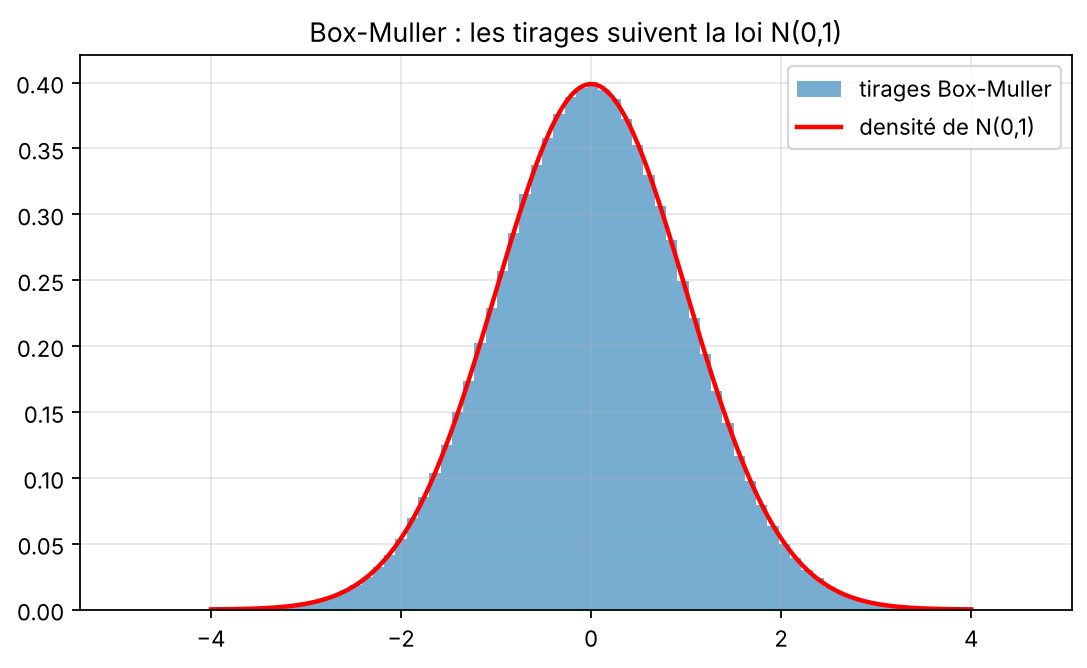
\includegraphics[width=0.7\textwidth]{fig_box_muller}
\caption{Un million de tirages de Box-Muller et la densité de la loi $\Ncal(0,1)$.}
\label{fig:bm}
\end{figure}

\section{Propriétés de l'estimateur}

\begin{demo}[ — sans biais, convergence, intervalle de confiance]
\textbf{Sans biais.} $\E[\hat C] = \frac1N\sum_i\E[Y_i] = C$.

\textbf{Convergence.} Les $Y_i$ sont indépendants et de même loi ; par la loi des grands nombres, $\hat C\to C$ quand $N\to\infty$.

\textbf{Variance.} Par indépendance, $\Var(\hat C) = \frac{\sigma_Y^2}{N}$ : l'erreur typique vaut $\sigma_Y/\sqrt N$.

\textbf{Intervalle de confiance.} Par le théorème central limite, $\sqrt N(\hat C-C)/\sigma_Y$ suit approximativement la loi $\Ncal(0,1)$. Comme $\Q(|\Ncal(0,1)|\le1{,}96) = 0{,}95$, et en remplaçant $\sigma_Y$ inconnu par l'écart-type empirique $s$ (calculé avec $N-1$ au dénominateur) :
\[
IC_{95\%} = \Big[\hat C - 1{,}96\frac{s}{\sqrt N}\ ;\ \hat C + 1{,}96\frac{s}{\sqrt N}\Big].
\]
\end{demo}

\begin{retenir}
La demi-largeur de l'IC décroît en $1/\sqrt N$ : pour diviser l'erreur par 10, il faut \textbf{100 fois plus} de simulations. Pour réduire l'erreur $1{,}96\,\sigma_Y/\sqrt N$, on peut augmenter $N$ (coûteux) ou diminuer $\sigma_Y$ : c'est la réduction de variance (section~\ref{sec:rv}).
\end{retenir}

\section{Résultats du Monte-Carlo standard}

On note $SE = s/\sqrt N$ l'\textbf{erreur standard} (l'écart-type de l'estimateur) ; l'IC à 95 \% est $\hat C\pm1{,}96\,SE$.

\textbf{Exemple à la main.} $Z = +1$ donne $S_T = 100\,e^{0{,}03+0{,}2} = 125{,}86$ et un payoff actualisé de $25{,}86\,e^{-0{,}05} = 24{,}60$. $Z = -1$ donne $S_T = 84{,}37<K$ et un payoff nul.

\textbf{Avec $N = 10^6$ simulations :}
\[
\hat C_{MC} = 10{,}4370,\qquad SE = 0{,}01471,\qquad IC_{95\%} = [10{,}4081\ ;\ 10{,}4658],\qquad \CBS = 10{,}4506\in IC.
\]
\textbf{Erreur par rapport au prix analytique :} $|\CBS - \hat C_{MC}| = 0{,}013624$.

\begin{figure}[H]
\centering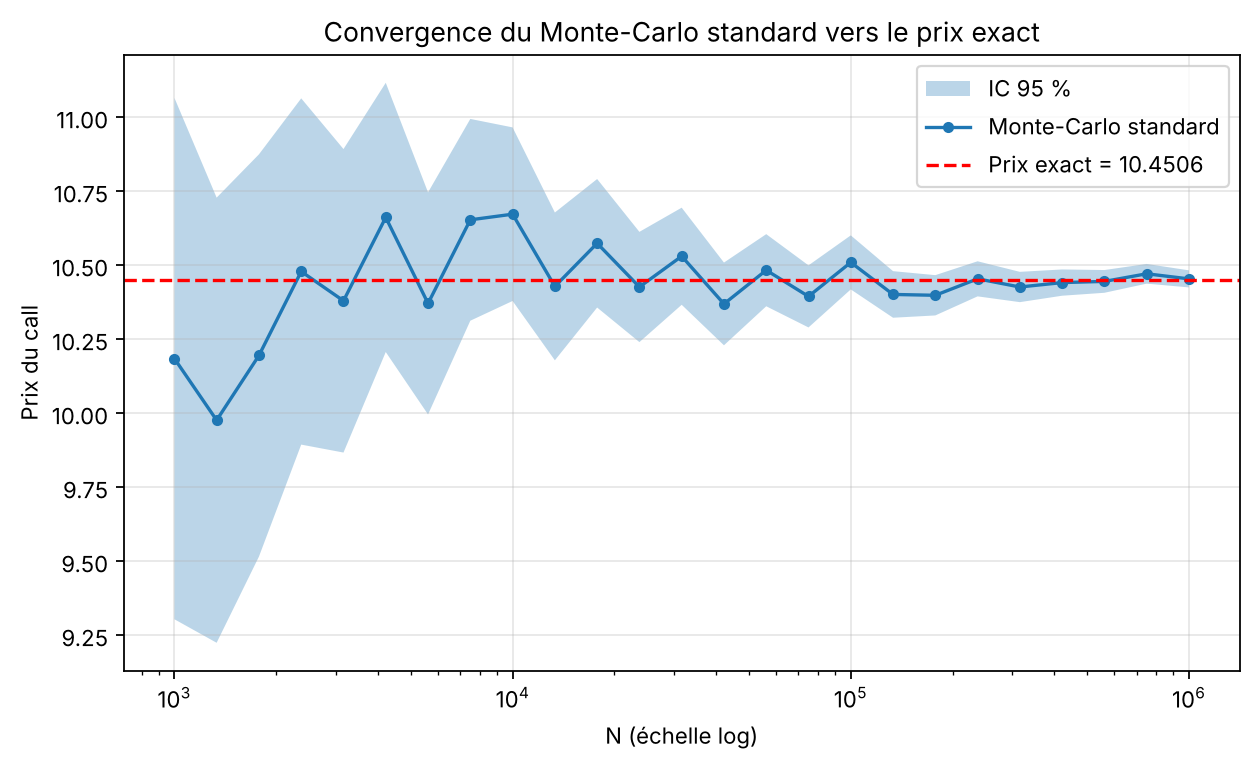
\includegraphics[width=0.82\textwidth]{fig_ic_vs_N}
\caption{Prix Monte-Carlo et IC à 95 \% pour 25 valeurs de $N$ entre $10^3$ et $10^6$.}
\label{fig:icN}
\end{figure}

\textbf{Lecture.} Quand $N$ augmente, l'intervalle se resserre autour de $10{,}4506$ : c'est la convergence de Monte-Carlo. Pour les 25 valeurs de $N$, le prix exact est dans l'IC. La largeur suit la loi $1/\sqrt N$ : multiplier $N$ par 1\,000 divise l'IC par environ $\sqrt{1000}\approx31{,}6$.

\subsection*{Prix pour les puissances de 10}
\begin{table}[H]
\centering\small
\begin{tabular}{rccc}
\toprule
$N$ & Prix MC & IC à 95 \% & Erreur $|\CBS - \hat C|$ \\
\midrule
10 & 11,9906 & [3,8810 ; 20,1002] & 1,5400 \\
100 & 10,1197 & [7,1120 ; 13,1275] & 0,3309 \\
1\,000 & 10,4897 & [9,5733 ; 11,4061] & 0,0391 \\
10\,000 & 10,5740 & [10,2834 ; 10,8645] & 0,1234 \\
100\,000 & 10,4234 & [10,3326 ; 10,5141] & 0,0272 \\
1\,000\,000 & 10,4371 & [10,4083 ; 10,4660] & 0,0134 \\
\bottomrule
\end{tabular}
\caption{Monte-Carlo standard pour $N = 10^1, \dots, 10^6$.}
\end{table}
À chaque puissance de 10, l'IC est divisé par environ $\sqrt{10}\approx3{,}16$ et contient toujours $\CBS$. L'erreur d'une seule simulation dépend du hasard (elle est plus grande à $10^4$ qu'à $10^3$) ; c'est la largeur de l'IC qui diminue toujours.

\subsection*{Trajectoire de l'estimateur : stabilité}
On suit la moyenne des $n$ premiers payoffs, $\hat C_n = \frac1n\sum_{i\le n}Y_i$, pour $n$ de 1 à $10^6$ (une seule simulation).
\begin{figure}[H]
\centering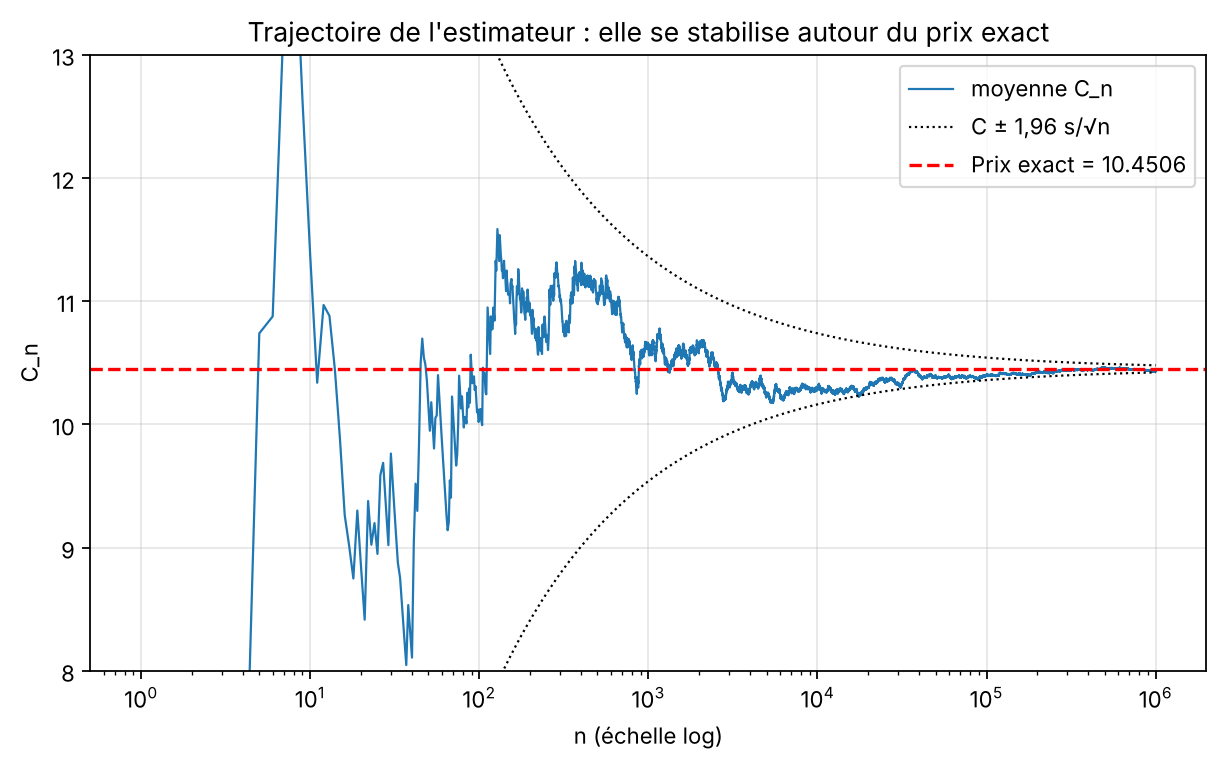
\includegraphics[width=0.82\textwidth]{fig_trajectoire}
\caption{Trajectoire $\hat C_n$ et enveloppe $\CBS\pm1{,}96\,s/\sqrt n$.}
\label{fig:traj}
\end{figure}
La moyenne bouge beaucoup au début ($\hat C_{1000} = 10{,}6402$), puis se stabilise dans l'enveloppe ($\hat C_{10^6} = 10{,}4308$) : c'est la loi des grands nombres.

\section{Réduction de variance}\label{sec:rv}

On remplace $Y$ par une autre variable \textbf{de même espérance} $C$ mais \textbf{de plus petite variance}. Toutes les méthodes sont comparées \emph{à budget égal} : $N$ payoffs chacune.

\subsection{Méthode 1 : les variables antithétiques}

Pour chaque tirage $Z$, on utilise aussi $-Z$, qui a exactement la même loi. On tire $N/2$ valeurs $Z_i$ (donc $N$ payoffs au total) et on pose $Y^+ = Y(Z)$, $Y^- = Y(-Z)$ :
\[
\hat C_{a} = \frac{1}{N/2}\sum_{i=1}^{N/2}\frac{Y^+_i+Y^-_i}{2}.
\]

\begin{demo}[ — biais et variance de l'estimateur antithétique]
\textbf{Sans biais.} $-Z$ a la même loi que $Z$, donc $\E[Y^-] = \E[Y^+] = C$ et $\E[\hat C_a] = C$.

\textbf{Variance.} Avec $\rho = \Corr(Y^+,Y^-)$ :
\[
\Var\Big(\frac{Y^++Y^-}{2}\Big) = \frac14\big(\sigma_Y^2+\sigma_Y^2+2\rho\sigma_Y^2\big) = \frac{\sigma_Y^2}{2}(1+\rho).
\]
Avec $N/2$ paires indépendantes : $\Var(\hat C_a) = \frac{\sigma_Y^2(1+\rho)}{N}$, donc
\[
\boxed{\text{gain}_{a} = \frac{\Var(\hat C_{MC})}{\Var(\hat C_a)} = \frac{1}{1+\rho}}.
\]
\textbf{Quand ça marche.} Il faut $\rho<0$. Le payoff du call augmente avec $Z$ : quand $Y^+$ est grand, $Y^-$ est petit, donc $\rho<0$.
\end{demo}

\textbf{Résultat ($N = 10^6$).} $\hat C_a = 10{,}4600$, $SE = 0{,}01039$ contre $0{,}01471$ en standard : gain de variance $(0{,}01471/0{,}01039)^2 = 2{,}00$, ce qui correspond à $\rho\approx-0{,}50$. Erreur par rapport au prix analytique : $|\CBS - \hat C_a| = 0{,}009445$.

\textbf{Pourquoi le gain n'est que de 2.} Le payoff du call est \emph{convexe} : il est nul quand $Z$ est négatif, puis croît comme une exponentielle. Quand $Z$ est grand, $Y^+$ est grand et $Y^- = 0$ : la paire ne se compense pas. La corrélation n'est que de $-0{,}5$, d'où un gain de 2.

\subsection{Méthode 2 : la variable de contrôle et le calcul de $c$}

On utilise une variable $X$ \textbf{corrélée} au payoff $Y$ dont on connaît \textbf{exactement} l'espérance : $X = S_T$, avec $\E[S_T] = S_0e^{rT}$ (chapitre 2). Pour un réel $c$ :
\[
Y_c = Y - c\,\big(X-\E[X]\big).
\]
\textbf{Idée.} Quand $S_T$ dépasse sa moyenne, le payoff est probablement grand aussi : on retire cet excès « prévisible ». Il reste à choisir combien retirer, c'est-à-dire $c$.

\begin{demo}[ — comment on trouve $c$]
\textbf{Sans biais pour tout $c$.} $\E[Y_c] = \E[Y] - c\big(\E[X]-\E[X]\big) = C$.

\textbf{La variance est un polynôme de degré 2 en $c$.}
\[
g(c) = \Var(Y_c) = \Var Y - 2c\,\Cov(Y,X) + c^2\Var X.
\]
\textbf{Minimisation.} $g'(c) = -2\Cov(Y,X) + 2c\Var X = 0$ donne
\[
\boxed{c^* = \frac{\Cov(Y,X)}{\Var(X)}},
\]
et $g''(c) = 2\Var X>0$ : c'est bien un minimum.

\textbf{Variance minimale.} En remplaçant : $g(c^*) = \Var Y - \frac{\Cov(Y,X)^2}{\Var X} = (1-\rho_{XY}^2)\Var Y$, donc
\[
\boxed{\text{gain}_{c} = \frac{1}{1-\rho_{XY}^2}},\qquad \rho_{XY} = \Corr(Y,X).
\]
\end{demo}

\paragraph{Calcul de $c$ pour le call.} Dans le code, $\Cov(Y,X)$ et $\Var(X)$ sont calculées sur les $N$ simulations (\texttt{np.cov} et \texttt{np.var}), puis $c^* = \Cov/\Var$ :
\[
c^* = 0{,}640505.
\]
\textbf{Vérification par le calcul exact.} Avec la loi log-normale de $S_T$ on peut calculer $c^*$ exactement : $\E[S_T\1_{S_T>K}] = S_0e^{rT}N(d_1)$, $\E[S_T^2\1_{S_T>K}] = S_0^2e^{(2r+\sigma^2)T}N(d_1+\sigma\sqrt T)$, $\Var(S_T) = S_0^2e^{2rT}(e^{\sigma^2T}-1)$, puis $\Cov(Y,S_T) = e^{-rT}\big(\E[S_T^2\1_{S_T>K}] - K\,\E[S_T\1_{S_T>K}]\big) - \CBS\,\E[S_T]$. On obtient $c_{\text{analytique}} = 0{,}640762$.
\[
\text{Erreur sur } c :\quad |c_{\text{analytique}} - c^*| = 0{,}000257\ (0{,}04\ \%) : \text{la valeur simulée est juste.}
\]

\textbf{Remarque.} Estimer $c$ sur les mêmes tirages que le prix crée un biais de l'ordre de $1/N$ ; avec $N = 10^6$ il est négligeable devant l'erreur standard.

\textbf{Résultat ($N = 10^6$).} $\hat C_c = 10{,}4472$, $SE = 0{,}00562$, $IC_{95\%} = [10{,}4362\ ;\ 10{,}4582]$, qui contient $\CBS$, erreur $|\CBS - \hat C_c| = 0{,}003408$. Gain de variance $(0{,}01471/0{,}00562)^2 = 6{,}86$, ce qui correspond à $\rho_{XY}\approx0{,}92$.

\subsection{Comparaison : MSE, gain, temps et efficacité}

Les trois estimateurs sont calculés avec le même budget ($N = 10^6$ payoffs). On compare :
\begin{itemize}[nosep]
\item l'\textbf{erreur standard} $SE$ et l'\textbf{IC à 95 \%} ;
\item la \textbf{MSE} : les trois estimateurs sont sans biais, donc $MSE = \E[(\hat C - C)^2] = \Var(\hat C) = SE^2$ ;
\item le \textbf{gain de variance} $= SE_{MC}^2/SE^2$ : combien de fois moins de simulations il faut pour la même précision ;
\item le \textbf{temps} de calcul et l'\textbf{efficacité} $= \text{gain}\times t_{MC}/t$ : le gain réel une fois le temps payé (temps moyen sur 5 exécutions).
\end{itemize}

\begin{table}[H]
\centering\small
\begin{tabular}{lccccccc}
\toprule
Méthode & Prix & $SE$ & IC à 95 \% & MSE $=SE^2$ & Gain & Temps (s) & Efficacité \\
\midrule
Standard & 10,4370 & 0,01471 & [10,4081 ; 10,4658] & 0,000216 & $\times1{,}00$ & 0,039 & $\times1{,}0$ \\
Antithétique & 10,4600 & 0,01039 & [10,4397 ; 10,4804] & 0,000108 & $\times2{,}00$ & 0,022 & $\times3{,}5$ \\
Contrôle & 10,4472 & 0,00562 & [10,4362 ; 10,4582] & 0,000032 & $\times6{,}86$ & 0,056 & $\times4{,}7$ \\
\bottomrule
\end{tabular}
\caption{Comparaison à budget égal ($N = 10^6$). $\CBS = 10{,}4506$ est dans les trois IC. Les temps dépendent de la machine.}
\label{tab:rv}
\end{table}

\textbf{Lecture.}
\begin{itemize}[nosep]
\item Les trois IC contiennent le prix exact : les trois méthodes sont correctes.
\item L'antithétique divise la variance par 2, la variable de contrôle par 6,9 : l'IC du contrôle est 2,6 fois plus étroit que celui du standard.
\item L'antithétique est même plus rapide (elle tire deux fois moins de gaussiennes). La variable de contrôle coûte un peu plus de temps, mais reste la plus efficace.
\item \textbf{Quel estimateur choisir ?} Celui qui a la plus petite erreur standard : la \textbf{variable de contrôle}. On ne choisit pas sur l'écart $|\hat C - \CBS|$ d'une seule simulation : cet écart dépend du hasard, alors que $SE$ mesure la précision de la méthode.
\end{itemize}

\subsection{Courbe de comparaison des trois méthodes}
\begin{figure}[H]
\centering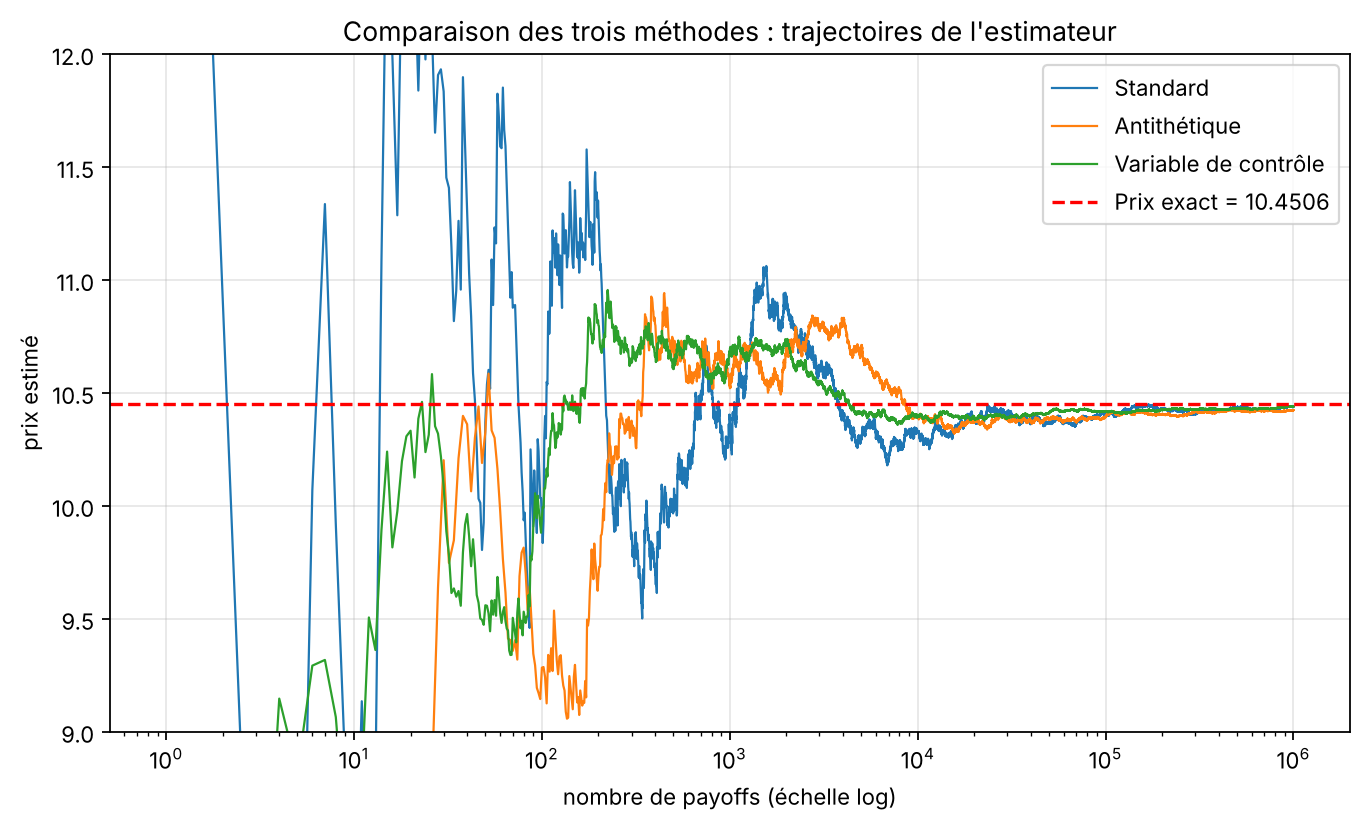
\includegraphics[width=0.82\textwidth]{fig_comparaison_3}
\caption{Moyenne cumulée de chaque méthode en fonction du nombre de payoffs (même budget).}
\label{fig:cmp3}
\end{figure}
Les trois trajectoires convergent vers $\CBS$ ; celle de la variable de contrôle oscille le moins.

\subsection{Prix pour les puissances de 10 : les trois méthodes}
\begin{table}[H]
\centering\small
\begin{tabular}{rcccccc}
\toprule
$N$ & Standard & erreur & Antithétique & erreur & Contrôle & erreur \\
\midrule
10 & 8,3558 & 2,0948 & 4,7035 & 5,7471 & 12,4296 & 1,9790 \\
100 & 7,6188 & 2,8318 & 10,2746 & 0,1760 & 10,9364 & 0,4858 \\
1\,000 & 10,3919 & 0,0587 & 10,4630 & 0,0124 & 10,0182 & 0,4324 \\
10\,000 & 10,2897 & 0,1609 & 10,4057 & 0,0448 & 10,5298 & 0,0793 \\
100\,000 & 10,4781 & 0,0275 & 10,4207 & 0,0299 & 10,4459 & 0,0046 \\
1\,000\,000 & 10,4486 & 0,0020 & 10,4693 & 0,0187 & 10,4516 & 0,0010 \\
\bottomrule
\end{tabular}
\caption{Prix et erreur $|\CBS - \hat C|$ des trois méthodes pour $N = 10^1, \dots, 10^6$.}
\end{table}
Pour $N$ petit, il y a trop peu de tirages et le prix peut être loin de $\CBS$. Quand $N$ grandit, les trois prix s'en rapprochent. Une seule simulation ne suffit pas pour comparer la précision : on répète donc le calcul à $N$ fixé.

\subsection{Stabilité des trois méthodes à $N = 10^6$ fixé}
On refait le calcul $M = 50$ fois avec chaque méthode ($N = 10^6$, nouveaux tirages à chaque fois). L'\textbf{erreur moyenne} est $\frac{1}{50}\sum_{j=1}^{50}|\CBS - \hat C_j|$.
\begin{figure}[H]
\centering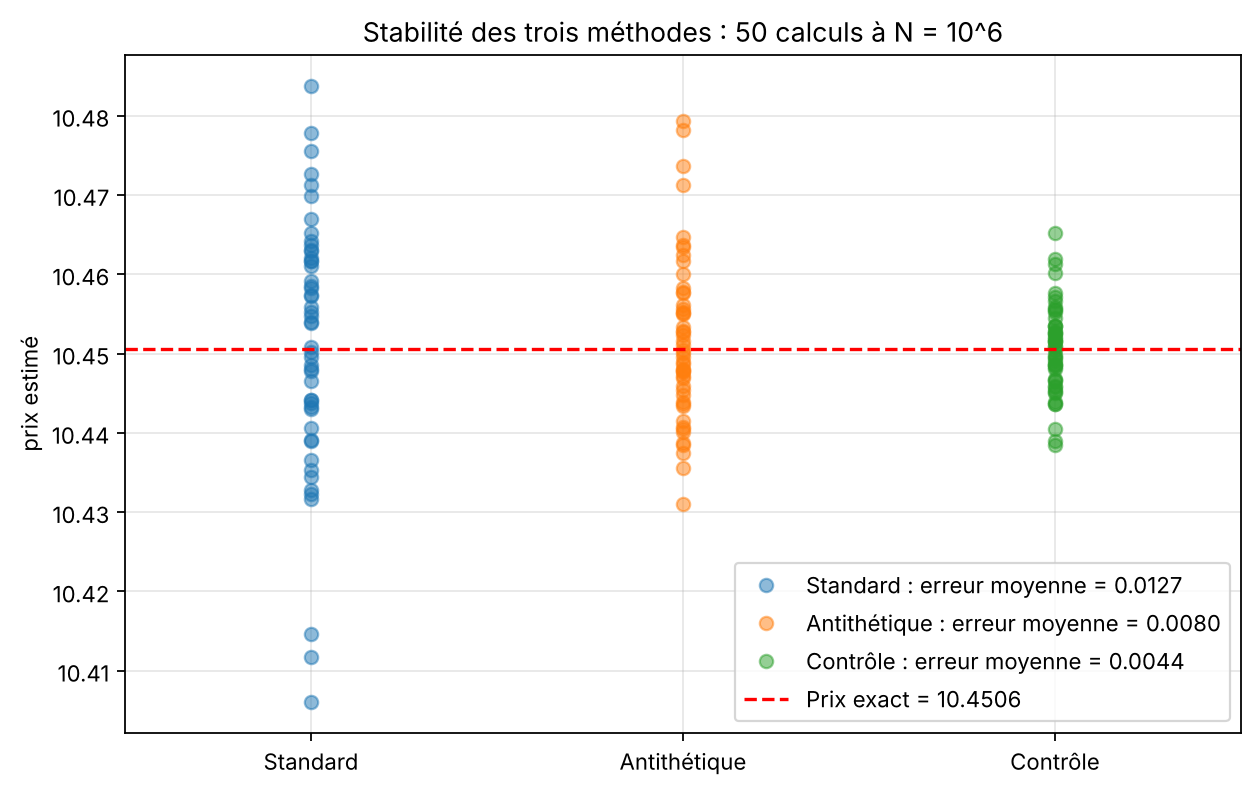
\includegraphics[width=0.78\textwidth]{fig_stabilite_3}
\caption{Les 50 prix de chaque méthode ; la ligne rouge est le prix exact.}
\label{fig:stab}
\end{figure}
\begin{table}[H]
\centering\small
\begin{tabular}{lccc}
\toprule
Méthode & Moyenne des 50 prix & Écart-type & \textbf{Erreur moyenne} \\
\midrule
Standard & 10,4512 & 0,01619 & \textbf{0,01265} \\
Antithétique & 10,4517 & 0,01052 & \textbf{0,00800} \\
Contrôle & 10,4507 & 0,00567 & \textbf{0,00440} \\
\bottomrule
\end{tabular}
\caption{Stabilité à $N = 10^6$ fixé (50 répétitions).}
\end{table}
Les trois colonnes sont centrées sur $\CBS$ (pas de biais). La variable de contrôle est la plus stable : son erreur moyenne est environ 3 fois plus petite que celle du standard. L'écart-type des 50 prix est proche du $SE$ calculé une seule fois, ce qui confirme les intervalles de confiance.

\subsection{La courbe de gain}

\begin{figure}[H]
\centering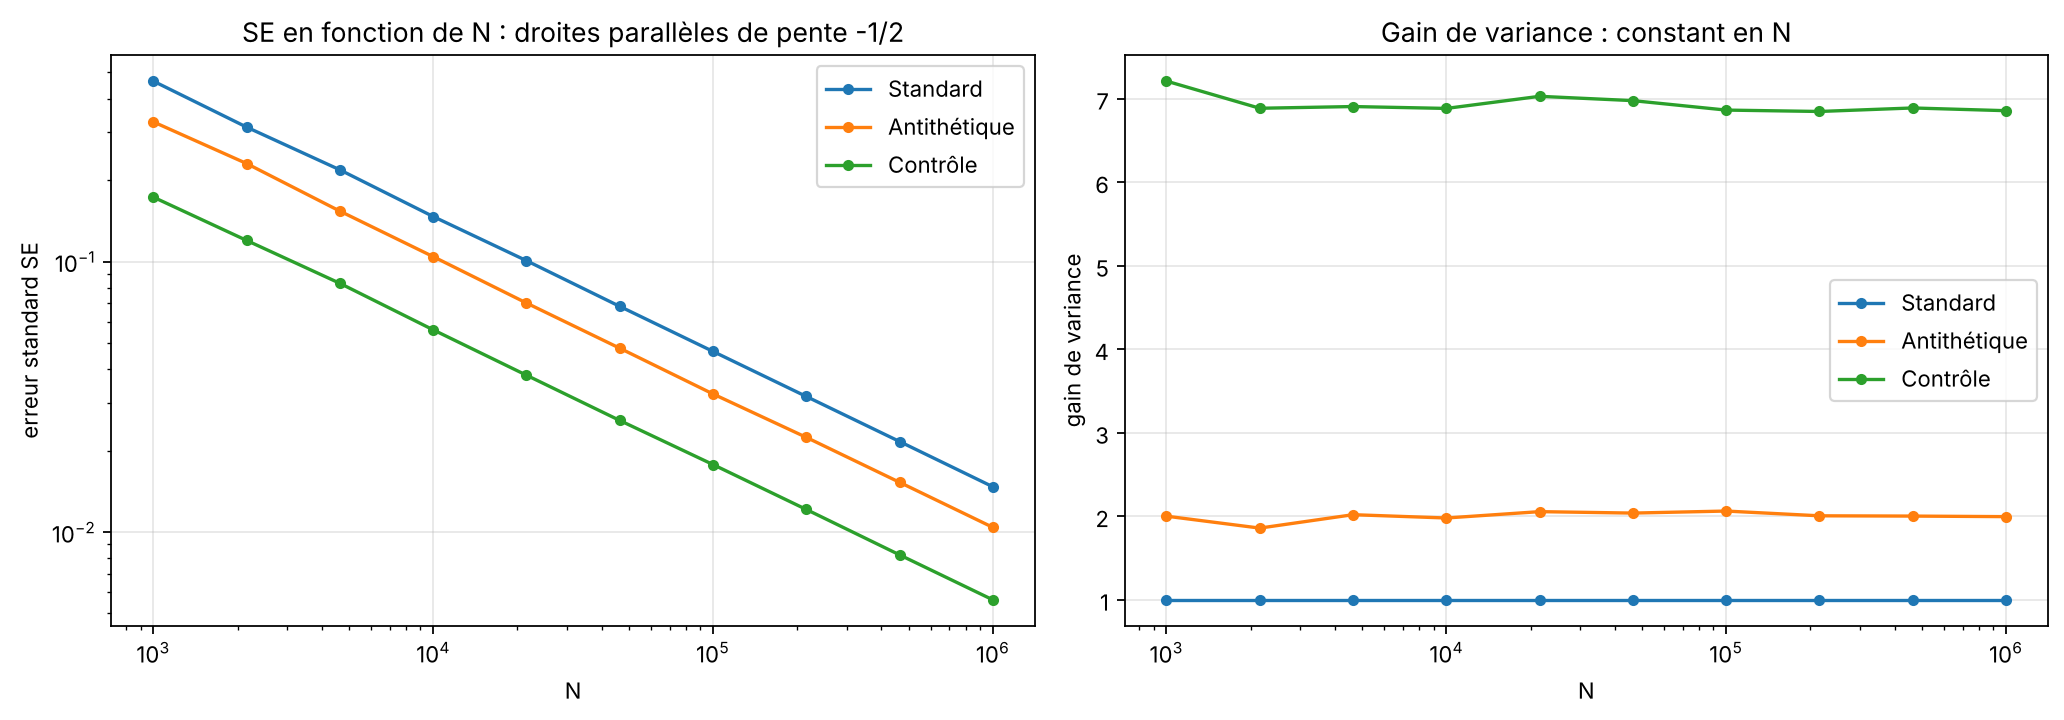
\includegraphics[width=\textwidth]{fig_courbe_gain}
\caption{Gauche : erreur standard des trois méthodes en fonction de $N$ (log-log). Droite : gain de variance en fonction de $N$.}
\label{fig:gain}
\end{figure}

\begin{question}{pourquoi avoir tracé une courbe de gain ?}
Le gain répond à la question pratique : \emph{combien de simulations économise-t-on ?} Un gain de 7 signifie que la méthode atteint avec $N$ simulations la précision que le Monte-Carlo standard atteint avec $7N$. La courbe montre deux choses :
\begin{enumerate}[nosep]
\item \textbf{à gauche}, trois droites \emph{parallèles de pente $-1/2$} : la réduction de variance \emph{ne change pas la vitesse} $1/\sqrt N$, elle \emph{abaisse la droite} d'un facteur $\sqrt{\text{gain}}$ ;
\item \textbf{à droite}, le gain est \emph{constant en $N$} (environ 2 pour l'antithétique, environ 7 pour le contrôle) car il ne dépend que de $\rho$.
\end{enumerate}
\end{question}

\begin{question}{pourquoi l'antithétique est-elle la plus basse ?}
Les deux gains dépendent d'une corrélation, mais pas de la même :
\begin{itemize}[nosep]
\item antithétique : gain $= 1/(1+\rho)$ avec $\rho = \Corr(Y^+,Y^-)\approx-0{,}50$, soit 2. Le payoff convexe empêche $Y^+$ et $Y^-$ de se compenser complètement ;
\item contrôle : gain $= 1/(1-\rho_{XY}^2)$ avec $\rho_{XY} = \Corr(Y,S_T)\approx0{,}92$, soit environ 7. Cette fonction augmente très vite quand $\rho$ s'approche de 1.
\end{itemize}
L'antithétique utilise seulement la \emph{symétrie} de la loi de $Z$ ; la variable de contrôle utilise une \emph{information en plus}, l'espérance exacte de $S_T$. Il est donc normal qu'elle fasse mieux.
\end{question}

\chapter{Implémentation : le code partie par partie}

Le code est le notebook \texttt{Projet\_MonteCarlo\_Call.ipynb}. Il est volontairement court : les paramètres sont des variables simples, les formules de $S_T$ et du payoff sont écrites directement dans chaque fonction, et il ne contient que ce que demande l'énoncé. Il s'exécute du début à la fin en une vingtaine de secondes et redonne exactement les chiffres de ce rapport. L'explication détaillée, ligne par ligne, est dans le document \emph{Explication du code}.

\begin{table}[H]
\centering\small
\begin{tabularx}{\textwidth}{>{\bfseries}p{1cm}p{5.2cm}L}
\toprule
Partie & Fonctions & Rôle \\
\midrule
1 & — & Imports, paramètres, générateur fixé \\
2 & \texttt{box\_muller} & Fabriquer les tirages $Z\sim\Ncal(0,1)$ \\
3 & \texttt{bs\_call} & Prix exact de Black-Scholes \\
4 & \texttt{mc\_call\_standard} & Méthode de base : prix, IC, erreur, puissances de 10, trajectoire \\
5 & \texttt{mc\_call\_antithetic} & Variables antithétiques \\
6 & \texttt{mc\_call\_control} & Variable de contrôle, $c^*$, $c$ analytique et erreurs \\
7 & — & Justification théorique \\
8 & — & Comparaison : tableau, courbe, puissances de 10, stabilité à $N$ fixé \\
9 & — & Courbe de gain \\
\bottomrule
\end{tabularx}
\caption{Plan du notebook.}
\end{table}

\section*{1. Imports et paramètres}
\addcontentsline{toc}{section}{1. Imports et paramètres}
\begin{lstlisting}
S0    = 100.0      # prix de l'action aujourd'hui
K     = 100.0      # prix d'exercice (strike)
T     = 1.0        # maturité : 1 an
r     = 0.05       # taux sans risque
sigma = 0.20       # volatilité
N     = 1_000_000  # nombre de simulations
rng = np.random.default_rng(2026)   # générateur fixé par une graine
z95 = 1.96                          # P(|Z| <= 1.96) = 95 %
\end{lstlisting}
Les cinq paramètres sont écrits une seule fois et utilisés directement par toutes les fonctions. Le générateur \texttt{rng} est créé une seule fois avec la graine 2026 : en exécutant le notebook du début à la fin, on obtient toujours les mêmes nombres.

\section*{2. Box-Muller}
\addcontentsline{toc}{section}{2. Box-Muller}
\begin{lstlisting}
def box_muller(n, rng):
    U1 = 1.0 - rng.random(n)          # uniforme sur ]0,1]
    U2 = rng.random(n)                # uniforme sur [0,1[
    return np.sqrt(-2.0 * np.log(U1)) * np.cos(2.0 * np.pi * U2)
\end{lstlisting}
Formule $Z = \sqrt{-2\ln U_1}\cos(2\pi U_2)$, démontrée au §\ref{sec:bm} : \textbf{une seule} gaussienne par couple d'uniformes. $1-U$ évite $\ln 0$. La cellule vérifie sur un million de tirages : moyenne $-0{,}0010$, variance $0{,}9987$, $\Q(|Z|\le1{,}96) = 0{,}9503$, et trace l'histogramme (figure~\ref{fig:bm}).

\section*{3. Black-Scholes}
\addcontentsline{toc}{section}{3. Black-Scholes}
\begin{lstlisting}
def bs_call():
    d1 = (np.log(S0 / K) + (r + sigma**2 / 2) * T) / (sigma * np.sqrt(T))
    d2 = d1 - sigma * np.sqrt(T)
    return S0 * norm.cdf(d1) - K * np.exp(-r * T) * norm.cdf(d2)
\end{lstlisting}
Formule démontrée au chapitre 2. \texttt{norm.cdf} est la fonction de répartition $N(x)$ de la loi $\Ncal(0,1)$ (bibliothèque \texttt{scipy}). Résultat : $\CBS = 10{,}4506$.

\section*{4. Monte-Carlo standard}
\addcontentsline{toc}{section}{4. Monte-Carlo standard}
\begin{lstlisting}
def mc_call_standard(N, rng):
    Z  = box_muller(N, rng)                                              # 1) tirages N(0,1)
    ST = S0 * np.exp((r - 0.5 * sigma**2) * T + sigma * np.sqrt(T) * Z)   # 2) prix finaux
    Y  = np.exp(-r * T) * np.maximum(ST - K, 0.0)                        # 3) payoffs actualisés
    prix = Y.mean()                                                      # 4) moyenne
    se   = Y.std(ddof=1) / np.sqrt(N)                                    #    erreur standard
    return prix, se
\end{lstlisting}
Les quatre étapes de l'algorithme, une ligne chacune. La ligne 2 est la solution exacte de l'EDS (chapitre 2) : pas d'erreur de discrétisation. \texttt{ddof=1} divise par $N-1$. L'IC est \texttt{prix} $\pm$ \texttt{z95*se}, et l'erreur est \texttt{abs(C\_exact - prix)}. Résultat pour $N = 10^6$ : $10{,}4370$, IC $[10{,}4081\ ;\ 10{,}4658]$, erreur $0{,}0136$. Les cellules suivantes tracent l'IC pour 25 valeurs de $N$ (figure~\ref{fig:icN}), le tableau des puissances de 10 et la trajectoire \texttt{np.cumsum(Y) / n} (figure~\ref{fig:traj}).

\section*{5. Variables antithétiques}
\addcontentsline{toc}{section}{5. Variables antithétiques}
\begin{lstlisting}
def mc_call_antithetic(N, rng):
    Z = box_muller(N // 2, rng)                                                  # N/2 tirages
    ST_plus  = S0 * np.exp((r - 0.5 * sigma**2) * T + sigma * np.sqrt(T) * Z)    # avec Z
    ST_minus = S0 * np.exp((r - 0.5 * sigma**2) * T - sigma * np.sqrt(T) * Z)    # avec -Z
    Y_plus   = np.exp(-r * T) * np.maximum(ST_plus - K, 0.0)
    Y_minus  = np.exp(-r * T) * np.maximum(ST_minus - K, 0.0)
    Y_anti   = (Y_plus + Y_minus) / 2                                            # moyenne de la paire
    prix = Y_anti.mean()
    se   = Y_anti.std(ddof=1) / np.sqrt(N // 2)
    return prix, se
\end{lstlisting}
$N/2$ tirages donnent $N$ payoffs : même budget que le standard. Les $N/2$ moyennes de paires sont indépendantes, d'où l'erreur standard calculée avec $\sqrt{N/2}$. Résultat : $10{,}4600$, $SE = 0{,}01039$, erreur $0{,}0094$.

\section*{6. Variable de contrôle et calcul de $c$}
\addcontentsline{toc}{section}{6. Variable de contrôle et calcul de c}
\begin{lstlisting}
def mc_call_control(N, rng):
    Z  = box_muller(N, rng)
    ST = S0 * np.exp((r - 0.5 * sigma**2) * T + sigma * np.sqrt(T) * Z)
    Y  = np.exp(-r * T) * np.maximum(ST - K, 0.0)
    X  = ST                                            # variable de contrôle
    EX = S0 * np.exp(r * T)                            # son espérance exacte
    c_star = np.cov(Y, X)[0, 1] / np.var(X, ddof=1)    # c* = Cov(Y,X) / Var(X)
    Y_c  = Y - c_star * (X - EX)                       # estimateur corrigé
    prix = Y_c.mean()
    se   = Y_c.std(ddof=1) / np.sqrt(N)
    return prix, se, c_star

# c analytique (loi log-normale de S_T)
c_analytique = cov_exact / var_exact
print(abs(c_analytique - c_star))                      # erreur sur c
\end{lstlisting}
\texttt{np.cov(Y, X)} renvoie la matrice de covariance de $(Y,X)$ ; son élément \texttt{[0, 1]} est $\Cov(Y,X)$. La formule $c^* = \Cov(Y,X)/\Var(X)$ est démontrée au chapitre 3, ainsi que $c_{\text{analytique}}$. Résultat : $c^* = 0{,}640505$, $c_{\text{analytique}} = 0{,}640762$, erreur $0{,}000257$ ; prix $10{,}4472$, $SE = 0{,}00562$, erreur $0{,}0034$.

\section*{7 à 9. Théorie, comparaison et courbe de gain}
\addcontentsline{toc}{section}{7 à 9. Théorie, comparaison et courbe de gain}
La partie 7 rappelle les démonstrations. La partie 8 reprend les trois résultats et affiche le tableau~\ref{tab:rv} (temps moyen sur 5 exécutions mesuré par \texttt{time.perf\_counter()}), trace la courbe de comparaison (figure~\ref{fig:cmp3}), le tableau des puissances de 10 pour les trois méthodes, puis répète 50 fois chaque méthode à $N = 10^6$ pour la stabilité et l'erreur moyenne (figure~\ref{fig:stab}). La partie 9 calcule l'erreur standard des trois méthodes pour 10 valeurs de $N$ et trace la courbe de gain (figure~\ref{fig:gain}).

\begin{retenir}
\textbf{Reproductibilité.} En exécutant le notebook de haut en bas (\emph{Kernel $\to$ Restart \& Run All}), on retrouve tous les nombres et toutes les figures de ce rapport. Seuls les temps de calcul varient d'une machine à l'autre.
\end{retenir}

\chapter*{Conclusion et perspectives}
\addcontentsline{toc}{chapter}{Conclusion et perspectives}
\markboth{Conclusion et perspectives}{}

\section*{Acquis}
\begin{itemize}
\item \textbf{Modèle.} Le modèle de Black-Scholes a été résolu par le lemme d'Itô ; la loi log-normale de $S_T$ donne la formule exacte du call, $\CBS = 10{,}4506$, qui sert de référence.
\item \textbf{Méthodes.} Chaque méthode de valorisation a été détaillée. Monte-Carlo est la plus lente sur ce cas simple, mais la seule dont l'erreur ne dépend pas de la dimension du problème.
\item \textbf{Box-Muller.} Les tirages gaussiens sont fabriqués à partir d'uniformes par la formule $Z = \sqrt{-2\ln U_1}\cos(2\pi U_2)$, démontrée et vérifiée (moyenne $-0{,}0010$, variance $0{,}9987$).
\item \textbf{Monte-Carlo de base.} L'estimateur retrouve $\CBS$ ($10{,}4370\pm0{,}0288$ pour $N = 10^6$, l'IC contient $\CBS$, erreur $0{,}0136$) et l'intervalle de confiance se resserre en $1/\sqrt N$.
\item \textbf{Optimisation.} À budget égal, l'antithétique divise la variance par environ 2 ; la variable de contrôle $S_T$, avec $c^* = \Cov(Y,S_T)/\Var(S_T) = 0{,}6405$ (valeur analytique $0{,}6408$, erreur $0{,}00026$), la divise par 6,9. Répétée 50 fois à $N = 10^6$, c'est aussi la plus stable (erreur moyenne $0{,}0044$ contre $0{,}0127$ en standard) : c'est l'estimateur le plus précis et le plus efficace.
\end{itemize}

\section*{Perspectives : la phase suivante}
\begin{itemize}[nosep]
\item Appliquer le simulateur validé ici à l'\textbf{option asiatique}, dont le payoff dépend de la moyenne des prix sur la trajectoire et qui n'a pas de formule fermée : simulation de la grille temporelle complète, sensibilité du prix au nombre de dates $M$ et au nombre de trajectoires $N$.
\item Combiner les méthodes de réduction de variance (antithétique et contrôle ensemble), ou utiliser des suites quasi-aléatoires (Sobol).
\item Remplacer Black-Scholes par Heston ou Merton : le code Monte-Carlo reste le même, seule la simulation de $S_T$ change.
\end{itemize}

\begin{thebibliography}{9}
\addcontentsline{toc}{chapter}{Bibliographie}
\bibitem{bs} F. Black et M. Scholes, \emph{The Pricing of Options and Corporate Liabilities}, Journal of Political Economy, 81(3), 637--654, 1973.
\bibitem{merton} R. C. Merton, \emph{Theory of Rational Option Pricing}, Bell Journal of Economics and Management Science, 4(1), 141--183, 1973.
\bibitem{glasserman} P. Glasserman, \emph{Monte Carlo Methods in Financial Engineering}, Springer, 2004.
\bibitem{crr} J. Cox, S. Ross et M. Rubinstein, \emph{Option Pricing: A Simplified Approach}, Journal of Financial Economics, 7, 229--263, 1979.
\bibitem{cm} P. Carr et D. Madan, \emph{Option Valuation Using the Fast Fourier Transform}, Journal of Computational Finance, 2(4), 61--73, 1999.
\bibitem{lapeyre} B. Lapeyre, É. Pardoux et R. Sentis, \emph{Méthodes de Monte-Carlo pour les équations de transport et de diffusion}, Springer, 1998.
\bibitem{ks} I. Karatzas et S. Shreve, \emph{Brownian Motion and Stochastic Calculus}, Springer, 2\textsuperscript{e} édition, 1991.
\end{thebibliography}


\appendix
\chapter{Réponses aux remarques de l'encadrant}

Ce tableau indique, pour chaque remarque formulée sur la version précédente du rapport, ce qui a été modifié et où le trouver.

\begin{table}[H]
\centering\small
\begin{tabularx}{\textwidth}{>{\raggedright\arraybackslash}p{4.6cm}L>{\raggedright\arraybackslash}p{2.6cm}}
\toprule
Remarque & Ce qui a été fait & Où \\
\midrule
Présenter les \textbf{modèles avant les méthodes} & Le chapitre 2 présente d'abord les modèles du sous-jacent (avec leurs EDS) et Black-Scholes en détail ; les méthodes viennent ensuite. & Chap.~2 \\
\addlinespace
\textbf{Détailler les méthodes}, pas seulement les comparer & Chaque méthode a sa sous-section : principe, équations, application au call européen, limites. Le tableau comparatif n'arrive qu'à la fin. & Chap.~2, §2.4 \\
\addlinespace
Le critère 2 devient le \textbf{critère 1} & La forme du payoff (vanille / exotique) est le critère 1 ; l'instant d'exercice devient le critère 2. & Chap.~1, tab.~\ref{tab:criteres} \\
\addlinespace
Se \textbf{concentrer sur le call européen}, pas de put & Tout le projet porte sur le call. L'option asiatique est reportée à la phase suivante. & Tout le rapport \\
\addlinespace
\textbf{Fixer le générateur} de nombres aléatoires & Un seul générateur \texttt{default\_rng(2026)} créé au début : en exécutant le notebook du début à la fin, on retrouve les mêmes chiffres. & §3.2 ; notebook, partie 1 \\
\addlinespace
Utiliser la \textbf{méthode de Box-Muller}, avec \textbf{un seul $Z$} & $Z = \sqrt{-2\ln U_1}\cos(2\pi U_2)$ : une seule gaussienne par couple d'uniformes. Démonstration, exemple à la main, vérification sur un million de tirages. & §3.2 ; fig.~\ref{fig:bm} \\
\addlinespace
\textbf{Méthode de base, puis optimiser} ; simulation de $C$ ($S_0$, exponentielle) & Monte-Carlo standard en 4 étapes ($Z$, $S_T = S_0\exp(\dots)$, payoff, moyenne), puis antithétique et variable de contrôle. & §3.1, §3.4, §3.5 \\
\addlinespace
Monte-Carlo et réduction de variance dans \textbf{la même section} & Un seul chapitre : méthode de base, puis réduction de variance, puis comparaison. & Chap.~3 \\
\addlinespace
\textbf{Démontrer comment on trouve $c$} et \textbf{le calculer dans le code} & Démonstration : variance quadratique en $c$, dérivée nulle, $c = \Cov/\Var$, minimum. Le code calcule $c^* = \Cov(Y,X)/\Var(X) = 0{,}640505$ ; le calcul analytique donne $0{,}640762$, erreur $|c_{\text{analytique}} - c^*| = 0{,}000257$. & §3.5.2 ; notebook, partie 6 \\
\addlinespace
Expliquer pourquoi l'\textbf{antithétique est la plus basse} et \textbf{pourquoi la courbe de gain} & Gain $= 1/(1+\rho)$ avec $\rho\approx-0{,}50$, contre $1/(1-\rho^2)$ avec $\rho\approx0{,}92$ ; courbe de gain : droites parallèles et gain constant en $N$. & §3.5.4 ; fig.~\ref{fig:gain} \\
\addlinespace
Un \textbf{code simple et propre}, sans éléments en trop & Paramètres en variables simples (\texttt{S0}, \texttt{K}, \texttt{T}, \texttt{r}, \texttt{sigma} : pas de \texttt{o.T}), formules de $S_T$ et du payoff écrites directement dans chaque fonction (sans fonction intermédiaire), seulement ce que demande l'énoncé, en 9 parties courtes. Le meilleur estimateur est choisi sur l'erreur standard, pas sur l'écart d'une seule simulation. & Chap.~4 ; notebook \\
\addlinespace
\textbf{Erreur} par rapport à la valeur analytique, en valeur absolue & $|c_{\text{analytique}} - c^*|$ pour $c$, et $|\CBS - \hat C|$ pour le prix des trois méthodes. & §3.4, §3.5 \\
\addlinespace
\textbf{Puissances de $N$}, \textbf{trajectoire} et \textbf{stabilité} & Tableaux pour $N = 10, \dots, 10^6$ ; trajectoire $\hat C_n$ ; courbe de comparaison des trois méthodes ; 50 répétitions à $N = 10^6$ fixé avec l'erreur moyenne. & §3.4, §3.5 \\
\bottomrule
\end{tabularx}
\caption{Correspondance entre les remarques et les corrections.}
\end{table}

\textbf{Autres corrections.} L'ancien chapitre 2, qui répétait le chapitre 1, a été fusionné dans le chapitre 3. Le code LaTeX cassé (listing illisible) a été remplacé. Le terme « projet de fin d'études » a été corrigé (projet du module Mathématiques et Assurance). La bibliographie n'apparaît plus qu'une fois. L'annonce du plan correspond maintenant aux chapitres réels. Les nombres du rapport proviennent tous du notebook final, ce qui corrige les incohérences entre l'ancien tableau 1.9 et l'ancien tableau 2.3.


\end{document}
